\chapter{Stretch 3 Scheme (for all graphs)}
We now generalizes the stretch 3 scheme for complete graphs to generic graphs. To do this, we introduce routing on trees, landmarks and partial shortest path trees.

\subsection{Routing on Trees}
From Fraigniaud and Gavoille 2001 \cite{fraigniaudGavoille2001}, Thorup og Zwick 2001B \cite{thorupZwick2001b}, we have:

For every weighted tree $T$ with $n$ nodes there exists a labeled routing scheme that, given any destination label, routes optimally on $T$ from any source to the destination. The storage per node in $T$, the label size, and the header size are $O(log2 n/ log log n)$ bits. Given the information of a node and the label of the destination, routing decisions take constant time, by Lemma 3.3 \cite{compactNameIndepRouting}[37:6].

For a tree $T$ containing a node $v$, let $\mu(T, v)$ denote the routing information
stored at node $v$ and $\lambda(T, v)$ denote the destination label of $v$ in $T$ as defined by the
labeled routing scheme of Lemma 3.3 \cite{compactNameIndepRouting}[37:6].

\subsection{Landmarks}
Designate one color to be the landmark color. Let $L$ denote the set of nodes with this color. Because of the way coloring works we have that $|L| \leq 2 \sqrt{n}$ and that for every $v\in V$, $B(v)\cap L \neq \emptyset$.

For a node $v\in V$, let $\ell_v$ denote the closest landmark node in $B(v)$.

\subsection{Partial shortest path trees}
For any node $u$, let $T(u)$ denote a singlesource minimum-cost-path tree rooted at $u$. In a partial shortest path tree, every node $v$ maintains $\mu(T(u),v)$ if and only if $u \in B(v)$. Notice that the set of nodes that maintain $\mu(T(u),\dot)$ is a subtree of $T(u)$ that contains $u$.\\

%\begin{quote}[\texttt{Lemma 3.4}]
%    \textit{If $x \in B(y)$, then given the label $\lambda(T(x), y)$, node $x$ can
%    route to node $y$ along a minimum cost path.}
%\end{quote}
%TODO: Prove this

\texttt{Lemma 3.4}. \textit{If $x\in B(y)$, then given the label $\lambda(T(x),y)$, node $x$ can route to node $y$ along a min cost path.}

\texttt{Proof}. By Property 3.1 for any node $w$ on the min cost path of $T(x)$ between $x$ and $y$ we have $x\in B(w)$. Thus every node $w$ on this path maintains $\mu(T(x),w)$

\subsection{Storing}\label{subsec:storing}
Every node $u$ stores the following
\begin{enumerate}
    \item For every $w\in B(u)$, the name $w$ and the port name $u\rightarrow y$, where $(u\rightarrow y)$ is the port number to use to get to node $y$, which is the next hop on a min cost path from $u$ to $w$.
    \item For every landmark node $\ell \in L$, routing information $\mu(T(\ell),u)$ and label $\lambda(T(\ell),\ell)$ of the tree $T(\ell)$.
    \item For every node $x\in B(u)$, routing information $\mu(T(x),u)$ of the tree $T(x)$.
    \item For every node v such that $c(u) = h(v)$, store one of the following two options that produces the minimum cost path out of the two:
    \begin{enumerate}
        \item[a] Store the labels $<\lambda(T (\ell_v), \ell_v ), \lambda(T (\ell_v), v)>$. The routing path in this case would be from $u$ to $\ell_v \in B(v)$ using $\lambda(T (\ell_v), \ell_v)$ on the tree $T (\ell_v)$, and from $\ell_v$ to $v$ using $\lambda(T (\ell_v), v)$ on the same tree $T (\ell_v)$.

        \item[b] Let $P(u, w, v)$ be a path from u to v composed of a minimum cost path from $u$ to $w$, and of a minimum cost path from $w$ to $v$ with the followingproperties: $u \in B(w)$, and there exists an edge $(x, y)$ along the minimum cost path from $w$ to $v$ such that $x \in B(w)$ and $y \in B(v)$. If such paths exists, choose the lowest cost path $P(u, w, v)$ among all these paths and store the labels $<\lambda(T (u), w), x, (x \rightarrow y), \lambda(T (y), v)>$.\\
        The routing path in this case would be from $u$ to $w$ on $T(u)$ using $\lambda(T (u), w)$. This part is possible by Lemma 3.4 on $u \in B(w)$. Then from $w$ to $y$ since $x \in B(w)$ and the port number $(x \rightarrow y)$ is stored. Finally from $y$ to $v$ on $T(y)$ using $\lambda(T (y), v)$. This part is possible by Lemma 3.4 on $y \in B(v)$.
    \end{enumerate}
\end{enumerate}

\subsection{Routing}
Routing from u to v is done in the following manner:
\begin{enumerate}
    \item If $v \in B(u)$ or $v \in L$ ($v$ is a landmark node) or $c(u) =
        h(v)$, then $u$ routes to $v$ using its own information.
    \item Otherwise, $u$ forwards the packet to $w \in B(u)$ such that
        $c(w) = h(v)$. Then from $w$ the packet goes to $v$ using $w$’s
        routing information.
\end{enumerate}

\section{Theorem 3.5}
\textit{Let $s,t\in V$ be any two nodes. The route of the scheme from $s$ to $t$ has stretch at most 3.}

\texttt{Proof}. There are three cases to consider:
\subsection{Analysis}
\begin{enumerate}
    \item \textit{The taget is inside the source vicinity}: If $t\in B(s)$ or $t\in L$, then $s$ routes on a minimum cost path directly to $t$.

    Otherwise, let $z$ be a node such that $z\in B(s)$ and $c(z)=h(t)$. For the case $c(s)=h(t)$, set $z=s$. Let $p(z,t)$ be the cost of the path chosen by $z$ as the lowest cost   path from $z$ to $t$ (from options 4(a) and 4(b)). Then:
    \item \textit{The source and target vicinities are far apart}: On every min cost path from $s$ to $t$ there is a node $y$ such that $y\not\in B(s)$ and $y\not\in B(t)$. In this case, $b(s)+b(t)\leq d(s,t)$.

    From 4(a) the cost $d(s,z)+p(z, t)$ of the path taken by the routing scheme is bounded by the cost of the path $s\leadsto z\leadsto \ell_t\leadsto t$, where $u\leadsto v$ is the min cost path from $u$ to $v$.\\
    Thus $d(s,z)+p(z,t) \leq d(s,z)+d(z,\ell_t)+d(\ell_t,t) \leq b(s) + [b(s) + d(s,t) + b(t)] + b(t) \leq 3d(s,t)$.
    \item \textit{The source and atarget vicinities are close}: There exists a min cost path in which every node is in $B(s)\cup B(t)$. Let $(x,y)$ be an edge on this path such that $x\in B(s)$ and $y\in B(t)$. From 4(b), the cost $d(s,z)+p(z,t)$ of the path taken is bounded by the cost of path $s\leadsto z\leadsto x\rightarrow y \leadsto t$.\\
    Thus $d(s,z)+p(z,t) \leq d(s,z) + d(z,s) + d(s,t) \leq b(s)+b(s)+d(s,t)\leq 3d(s,t)$.
\end{enumerate}
The three cases is depicted in \autoref{fig:threecases}.

\begin{figure}[htbp]
    \centering
    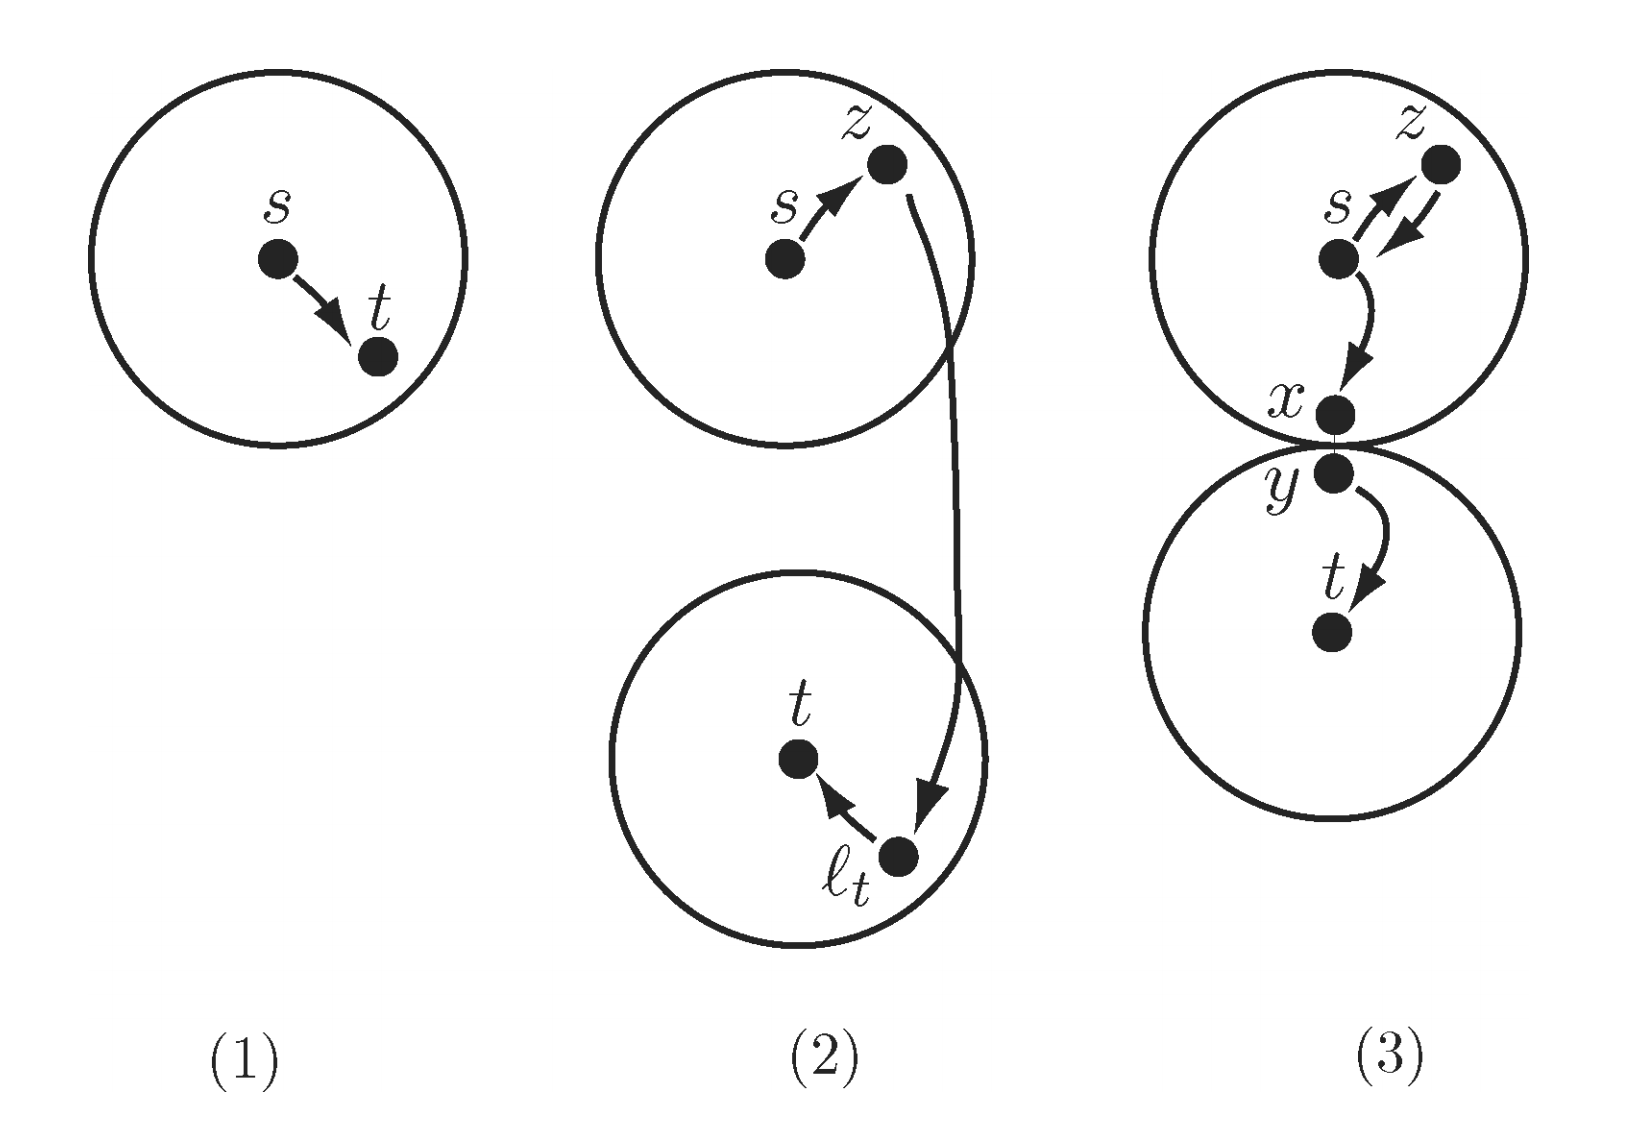
\includegraphics[scale=0.3]{images/threecases.png} 
    \caption{An illustration of the three cases described in the analysis.}
    \label{fig:threecases}
\end{figure}


\section{Results}
The routing information stored at each node in \ref{subsec:storing} is bounded by
\begin{enumerate}
    \item $\tilde{O}(\sqrt{n})$ as $|B(u)| = \tilde{O}(\sqrt{n})$.
    \item $\tilde{O}(\sqrt{n})$ as each node will participate in $\tilde{O}(\sqrt{n})$ trees and thus its total tree routing information is of size $\tilde{O}(\sqrt{n})$ by Lemma 3.3.
    \item $\tilde{O}(\sqrt{n})$ by the same logic as for the above.
    \item $\tilde{O}(\sqrt{n})$ as for a node $u$ the number of nodes $v$ such that $c(u) = h(v)$ is bound by $\tilde{O}(\sqrt{n})$ (by the property 3.2 and the assumption of the hashing being balanced), and the lables stored are of $\tilde{O}(1)$ size.
\end{enumerate}
giving the a total bound on size of $\tilde{O}(\sqrt{n})$.

The described stretch 3 scheme has the following bounds:
\begin{description}
    \item[Stretch] 3
    \item[Header size] $O(log^2/log\;log\;n)$ bits
    \item[Routing information stored per node] $\tilde{O}(\sqrt{n})$ bits
    \item[Routing] $O(1)$ time
    \item[Construction time] $\tilde{O}(n|E|)$
\end{description}
where the routing information stored per node 

Improves the stretch of Arias et al. [2003]\cite{ariasEtAl2003} from 5 to 3, the known lower bound and answers the open problem from 1989 [Awerbuch et al. 1990]. %TODO cite
